\chapter{Simulation Environment}
\label{ch:environment}
\section{Genesis: The Simulator}
\label{sec:genesis}

Every quantity optimized in this thesis is measured in simulation. A body is scored by flying it, a controller is trained by flying it, and the searches of the following chapters fly about a quarter of a million drones in every generation. The simulator is therefore the component that decides which experiments are affordable at all, and its internal organization leaves visible marks on the method. This work uses \emph{Genesis} \cite{genesis2024}, an open-source physics engine for robotics released in December 2024, in its version 0.3.7. Genesis is written entirely in Python, but its numerical core is compiled at run time into code for the Graphics Processing Unit (GPU), so that tens of thousands of independent copies of the same scene advance in parallel on a single card. Genesis has no model of the air: the forces that keep a winged drone aloft are computed by a custom aerodynamic solver that is not part of the public release, was developed outside this thesis (it is credited in \autoref{subsec:genesis-aero}) and runs inside the engine next to its rigid body solver.

This section describes how Genesis is organized and how its code reaches the GPU, weighs what that design gives and what it costs, and then follows one simulation step through its two halves: the rigid body dynamics that Genesis provides and the aerodynamic forces that were added to it. It closes with the random perturbations that are injected into both.

\subsection{Architecture and Taichi Kernels}
\label{subsec:genesis-architecture}

A Genesis program builds a \emph{scene}. The scene owns a \emph{simulator}, and the simulator owns a set of \emph{solvers}, one for each physical model the engine supports: articulated rigid bodies, and a family of continuum models for liquids, granular media, cloth and deformable solids (the material point method, smoothed particle hydrodynamics, finite elements, position based dynamics and a grid based fluid solver). A \emph{coupler} exchanges forces between solvers when objects of different kinds touch. The objects themselves are \emph{entities}, each defined by a \emph{morph} that gives its geometry (a primitive shape, a mesh, or a robot description file) and by a material that decides which solver is responsible for it. Only the solvers that own at least one entity are stepped. In this thesis the scene contains a single entity, the drone, loaded from a Unified Robot Description Format (URDF) file that is generated from the genome of the body; it is handled by the rigid body solver, and the aerodynamic solver acts on it as one more solver of the same simulator. Rendering is a separate subsystem and stays switched off during training and search.

None of the numerical work is done by the Python interpreter. Genesis is built on \emph{Taichi} \cite{hu2019taichi, hu2020difftaichi}, a domain specific language for parallel numerical computation that is embedded in Python, and of which the Genesis developers maintain their own fork. A Taichi \emph{kernel} is a function written in a statically typed subset of Python syntax and marked with a decorator. The first time a kernel is called, Taichi does not execute its body: it reads the syntax tree of the function, translates it into its own intermediate representation, applies the usual optimizations of a compiler (constant folding, elimination of common subexpressions and of dead branches, simplification of memory accesses) and lowers the result through LLVM to machine code for the selected backend, which here is CUDA. This is \emph{just-in-time} compilation: the program is compiled while it runs, the first time each piece is needed, and every later call launches the compiled binary directly (\autoref{fig:taichi-kernel}).

\begin{figure}[htbp]
\centering
\begin{tikzpicture}[
    >={Stealth[length=2mm]}, thick,
    every node/.style={font=\small},
    node distance=0.55cm,
]
\node[agentbox, align=center] (py) {Python function\\marked as kernel};
\node[affbox, align=center, right=1.5cm of py] (ast) {syntax\\tree};
\node[affbox, align=center, right=0.45cm of ast] (ir) {Taichi IR,\\optimization};
\node[affbox, align=center, right=0.45cm of ir] (llvm) {LLVM};
\node[envbox, align=center, right=0.45cm of llvm] (bin) {GPU\\binary};
\node[concatbox, align=center, above=0.7cm of bin] (cache) {on-disk cache};
\node[criticbox, align=center, below=1.2cm of ir, xshift=0.2cm] (launch) {launch: one GPU thread for each\\iteration of the outermost loop};

\draw[->] (py) -- node[above]{\scriptsize first call} (ast);
\draw[->] (ast) -- (ir);
\draw[->] (ir) -- (llvm);
\draw[->] (llvm) -- (bin);
\draw[<->] (bin) -- (cache);
\draw[->] (bin.south) |- (launch.east);
\draw[->] (py.south) |- node[above, pos=0.72]{\scriptsize later calls} (launch.west);
\end{tikzpicture}
\caption[Life of a Taichi kernel]{Life of a Taichi kernel. The first call compiles the Python function down to a GPU binary, which is also written to a cache on disk; later calls, and later runs of the same program, skip the compilation and only launch the binary. IR stands for intermediate representation.}
\label{fig:taichi-kernel}
\end{figure}

What makes a kernel parallel is a single rule: the outermost \texttt{for} loop of a kernel is parallelized automatically, and on a GPU every iteration of that loop becomes one thread. The body of the loop can be arbitrary scalar code, with branches, local variables, inner loops and calls to other Taichi functions, and all of it is fused into one GPU program. This is the opposite of the way a tensor library such as PyTorch reaches the GPU, where every elementary operation is a separate GPU program that reads and writes whole arrays. Physics code is full of logic that differs from element to element (a joint limit that is active in one copy of the scene and not in the next, a wing that is stalled here and not there), and it is awkward and wasteful to express as a chain of whole-array operations, while inside a kernel it is an ordinary \texttt{if}. Every kernel launch from Python has a small fixed cost, so the engine is organized as a few large kernels rather than many small ones.

The data that kernels work on live in \emph{fields}: typed, multidimensional arrays that are allocated on the GPU and declared separately from the kernels that use them. Keeping the description of the data apart from the computation is the central idea of Taichi \cite{hu2019taichi}, and it has a consequence that matters in practice. A kernel refers to its fields as global variables, so at compilation time it is bound to those specific fields and to their shapes; and the parameters that are declared static (the options of a solver, the number of links of a robot, which branches of the code are enabled) are compiled in as constants, with the unused branches removed. A compiled kernel is therefore specialized to one scene. Genesis makes this explicit by separating the construction of a scene from its \emph{build}: entities and options are declared first, and a single build call then allocates every field and fixes every static parameter. After the build, the values stored in the fields can change freely, which covers the state of the simulation and the physical parameters that were declared as varying, but nothing structural can: not the number of bodies, not their topology or geometry, not the size of any array. A structural change requires a new scene and a new build.

The most important structural parameter is the number of parallel \emph{environments} $B$, given to the build call. The $B$ environments are independent copies of the scene that share one model (the kinematic tree, the geometry, the nominal inertias) and differ in their state. Every state field has an axis of length $B$: the generalized positions form an array of size $n_q \times B$, the joint space inertia matrix an array of size $n_v \times n_v \times B$, and the parallel loop of each kernel runs over pairs (element, environment), so that a single launch advances every link of every environment. Environments never interact, which is exactly the structure of the workloads of this thesis: many flights of the same body, each in its own forest. Finally, the fields can be read and written as PyTorch tensors that reside on the same GPU: the exchange is a copy between two regions of the memory of the card and never passes through the host. The neural controllers, the obstacle fields and the reward computations are PyTorch code, the physics is Taichi code, and during a run only logging scalars ever leave the GPU.

\subsection{Advantages and Disadvantages}
\label{subsec:genesis-proscons}

The first reason to choose Genesis is throughput. The generalist controllers of this thesis are trained on 65\,536 simultaneous flights and a single generation of the body search scores 245\,760 of them; with the whole loop of physics, perception and control resident on the GPU, these sizes are reachable on one or two cards, and the costs reported in \autoref{tab:feasibility} are the measured result. The second reason is that the engine is open to extension at the level where it matters. Because a solver is a Python class whose numerical methods are Taichi kernels, a new physical model can be written in the same language as the engine, registered next to the built-in solvers, and compiled into the same GPU pipeline with direct access to the state of the rigid bodies. The aerodynamic solver used in this thesis is such an extension, and it evaluates the forces on every surface of every drone in one kernel launch per step. The same holds for perception: the depth sensor of the drone is a custom kernel that intersects rays with the trees of each environment. The third reason is the interface. Bodies are read from standard robot description files, which a script can generate from a genome; the state is exposed as batched PyTorch tensors, which is the format that reinforcement learning libraries expect; and physical parameters such as the masses and the centres of mass of the links can be perturbed independently in every environment. Lastly, Genesis is open source, so the whole stack can be packaged in a container and run unchanged on a workstation and on a cluster.

The costs follow from the same design. Compilation is slow: the first build of a scene compiles hundreds of kernels and can take several minutes, against the milliseconds of a simulation step. The cache on disk removes most of this cost from later runs, but a build still has to allocate and initialize the scene, and it is paid for every scene. This matters for co-design more than for ordinary robot learning, because all the environments of a scene share one body: a population of different bodies needs one scene per body, and replacing the bodies means building new scenes. Two further restrictions make this worse. Genesis can be initialized only once in a process and all its scenes share one Taichi runtime, so the scenes of a process are stepped one after the other; real parallelism across scenes is obtained with separate processes, each with its own share of the GPU memory. And since kernels are bound to their fields when they are compiled, a program that replaces a field after the first launch (for instance to change the number of trees) leaves the compiled kernel reading the old one, silently. Every array whose size might change has to be dimensioned for the worst case at build time, or its owner rebuilt.

Numerical precision is a second limitation. Genesis runs in 32-bit floating point by default, with the relaxed arithmetic rules that compilers use for speed, and the order in which parallel GPU threads accumulate sums is not guaranteed. Two runs with the same random seed do not produce the same trajectories: the differences start at the last bit and, because a flight among obstacles is a chaotic system, grow until the two flights end differently. The outcome of a flight must therefore be treated as a random variable even when every explicit source of randomness is held fixed, and a fitness value is only meaningful as an average over many flights.

Finally, Genesis is a young project. Its programming interface still changes between releases and parts of its documentation lag behind the code. For fixed-wing flight it offers nothing out of the box: its only aerial model is a quadrotor whose propellers produce a thrust proportional to the square of their rotation speed. Everything aerodynamic in this thesis comes from a solver added to the engine, and because an added solver exchanges forces with the rigid body solver explicitly, once per substep, its numerical stability has to be secured by a small time step and by limits on the forces, as described below.

\subsection{Physics Simulation}
\label{subsec:genesis-physics}

The drone is an articulated rigid body: a fuselage that moves freely in space and carries six revolute joints, driven by servomotors, which sweep and twist the two front wings and deflect the elevator and the rudder (the body is described in \autoref{sec:drone-model}). Its configuration $\vect{q}$ collects the position of the fuselage, its orientation as a unit quaternion and the six joint angles, for $n_q = 13$ numbers, and its generalized velocity $\vect{v}$ collects the linear and angular velocity of the fuselage and the six joint rates, for $n_v = 12$ degrees of freedom. The rigid body solver of Genesis follows the formulation of MuJoCo \cite{todorov2012mujoco}, and advances the equation of motion in generalized coordinates,
\begin{equation}
\mat{M}(\vect{q})\,\dot{\vect{v}} + \vect{c}(\vect{q}, \vect{v}) = \vect{\tau}_{\mathrm{act}} + \vect{\tau}_{\mathrm{pas}} + \mat{J}_{\mathrm{a}}(\vect{q})^{\top} \vect{F}_{\mathrm{a}} + \mat{J}_{\mathrm{c}}(\vect{q})^{\top} \vect{f}_{\mathrm{c}},
\label{eq:eom}
\end{equation}
where $\mat{M}$ is the joint space inertia matrix, $\vect{c}$ gathers the Coriolis, centrifugal and gravitational terms, $\vect{\tau}_{\mathrm{act}}$ and $\vect{\tau}_{\mathrm{pas}}$ are the actuator and the passive joint torques, $\vect{F}_{\mathrm{a}}$ stacks the aerodynamic forces with $\mat{J}_{\mathrm{a}}$ the Jacobian of their points of application, and $\vect{f}_{\mathrm{c}}$ are the constraint forces with Jacobian $\mat{J}_{\mathrm{c}}$. At every substep the solver computes $\mat{M}$ with the composite rigid body algorithm and $\vect{c}$ with the recursive Newton-Euler algorithm \cite{featherstone2008rigid}, both of which traverse the kinematic tree in a time linear in the number of links, and factorizes $\mat{M}$ once for all the linear systems that follow.

The servomotors are modelled as proportional-derivative position controllers with a bounded torque,
\begin{equation}
\tau_{\mathrm{act},j} = \operatorname{clip}\!\left( k_p \left(q_j^{\star} - q_j\right) - k_v\, v_j,\; -\tau_j^{\max},\; \tau_j^{\max} \right),
\label{eq:servo}
\end{equation}
with $k_p = 8$~N\,m/rad, $k_v = 2$~N\,m\,s/rad and a torque limit of 1.5~N\,m for the wing joints and 1~N\,m for the tail joints. The target angle $q_j^{\star}$ is what the controller commands. The passive torques are a viscous damping and a dry friction in each joint, and an armature term, which stands for the reflected inertia of the motor and of its gears, is added to the diagonal of $\mat{M}$. The response of a control surface to a command is thus not instantaneous: it is the response of a damped second order system with a saturating motor, and its delay is part of what the controller has to cope with.

Constraints are handled as in MuJoCo, by a convex optimization over accelerations rather than by a complementarity problem \cite{todorov2014convex}. Let $\vect{a}_0 = \mat{M}^{-1}(\vect{\tau}_{\mathrm{act}} + \vect{\tau}_{\mathrm{pas}} + \mat{J}_{\mathrm{a}}^{\top} \vect{F}_{\mathrm{a}} - \vect{c})$ be the acceleration the system would have without constraints. The solver selects
\begin{equation}
\begin{gathered}
\dot{\vect{v}} = \arg\min_{\vect{a}}\; \frac{1}{2}\,(\vect{a} - \vect{a}_0)^{\top} \mat{M}\, (\vect{a} - \vect{a}_0) \;+\; \sum_{i \,\in\, \mathcal{A}(\vect{a})} \frac{1}{2}\, d_i \left( \mat{J}_i\, \vect{a} - a_i^{\mathrm{ref}} \right)^2, \\
a_i^{\mathrm{ref}} = -b_i\, \mat{J}_i \vect{v} - k_i\, r_i ,
\end{gathered}
\label{eq:constraint-opt}
\end{equation}
that is, the acceleration closest to the unconstrained one in the metric of the kinetic energy (Gauss's principle of least constraint), softened by a penalty on each active constraint $i$. The reference acceleration $a_i^{\mathrm{ref}}$ is that of a critically damped spring which would bring the violation $r_i$ back to zero within a chosen time constant, the weight $d_i$ sets how stiffly the constraint is enforced, and the set $\mathcal{A}(\vect{a})$ contains the inequality constraints that are currently pushing in their admissible direction. The problem is convex and has a unique solution, and the constraint forces $\vect{f}_{\mathrm{c}}$ follow from it. Genesis offers a Newton and a conjugate gradient method for \eqref{eq:constraint-opt}; this thesis uses the latter. In the scenes of this work the problem is small, because contacts are disabled (see below): the only constraints are the mechanical limits of the six joints, which become active only when a joint reaches its stop, and the dry friction of the joints.

Time integration is semi-implicit Euler. With substep $\Delta t$,
\begin{equation}
\vect{v}_{k+1} = \vect{v}_k + \Delta t\, \dot{\vect{v}}_k, \qquad \vect{q}_{k+1} = \vect{q}_k \oplus \Delta t\, \vect{v}_{k+1},
\label{eq:integration}
\end{equation}
where the new velocity is used to advance the positions and $\oplus$ denotes ordinary addition for positions and joint angles and the composition with the rotation of axis and angle $\Delta t\,\vect{\omega}_{k+1}$ for the quaternion, which thereby stays of unit norm. The default integrator of Genesis, used here, makes one modification for stiff actuators: the joint damping $\mat{D}$ and the derivative gains $\mat{K}_v$ of the servomotors are treated implicitly, which amounts to replacing $\mat{M}$ with $\mat{M} + \Delta t\,(\mat{D} + \mat{K}_v)$ in the computation of the acceleration and keeps the servo loop stable whatever its gains. All other forces, the aerodynamic ones included, are explicit: they are evaluated on the state at the beginning of the substep and held constant across it.

Two time scales are used. The controller acts at 25~Hz, and every control step of 0.04~s is divided into four physics substeps of $\Delta t = 0.01$~s, so that the dynamics and the aerodynamic forces are updated at 100~Hz while commands are held (\autoref{fig:sim-step}). The finer physics step is what the explicit aerodynamic coupling requires: a lifting surface reacts to a change of incidence with a force that opposes it, which makes the equations stiff, and an explicit scheme remains stable only if the step is small compared with the fastest of these reactions.

\begin{figure}[htbp]
\centering
\begin{tikzpicture}[
    >={Stealth[length=2mm]}, thick,
    every node/.style={font=\small},
]
\node[agentbox, align=center] (ctrl) at (0,3.0) {controller\\(PyTorch)};
\node[affbox, align=center] (cmd) at (8.6,3.0) {servo targets $\vect{q}^{\star}$,\\throttle $u$};

\node[tanhbox, align=center] (aero) at (-0.4,0) {aerodynamic\\solver};
\node[affbox, align=center] (fd) at (2.9,0) {forward\\dynamics};
\node[affbox, align=center] (con) at (6.0,0) {constraint\\solver};
\node[affbox, align=center] (int) at (9.2,0) {integration,\\kinematics};

\node[envbox, align=center] (state) at (8.6,-3.0) {state tensors\\(no host copy)};
\node[envbox, align=center] (obs) at (1.2,-3.0) {forest tensors: depth rays,\\collision test, observations};

\begin{scope}[on background layer]
\node[draw=gray, dashed, rounded corners, fit=(aero)(fd)(con)(int), inner xsep=0.35cm, inner ysep=0.75cm] (sub) {};
\end{scope}
\node[anchor=south west, font=\scriptsize, text=gray!50!black] at (sub.north west) {physics substep, repeated 4 times (100 Hz)};

\draw[->] (ctrl) -- node[above]{\scriptsize every 0.04 s (25 Hz)} (cmd);
\draw[->] (cmd.south) -- (cmd.south |- sub.north);
\draw[->] (aero) -- node[above]{\scriptsize $\vect{F}_{\mathrm{a}}$} (fd);
\draw[->] (fd) -- node[above]{\scriptsize $\vect{a}_0$} (con);
\draw[->] (con) -- node[above]{\scriptsize $\dot{\vect{v}}$} (int);
\draw[->] (int.south) -- ++(0,-0.45) -| node[below, pos=0.25]{\scriptsize $\vect{q}, \vect{v}$} (aero.south);
\draw[->] (state.north |- sub.south) -- (state.north);
\draw[->] (state) -- (obs);
\draw[->] (obs.west) -| ([xshift=-1.7cm]ctrl.west) -- (ctrl.west);
\end{tikzpicture}
\caption[One control step of the simulation]{One control step. The commands of the controller are held while four physics substeps are executed; in each of them the aerodynamic solver turns the current state into forces, and the rigid body solver of Genesis computes the unconstrained acceleration, enforces the joint limits and integrates. Everything in the figure runs on the GPU, for all environments at once.}
\label{fig:sim-step}
\end{figure}

Genesis has a complete collision pipeline: a broad phase that sorts axis-aligned bounding boxes to discard distant pairs, a narrow phase for convex shapes, a convex decomposition for meshes that are not convex, and contact forces with Coulomb friction that enter \eqref{eq:constraint-opt} as further constraints. None of it is used here, and the trees of the forest are not objects of the physics engine at all. There are two reasons. A flight ends the moment the drone touches anything, so no contact ever has to be resolved, only detected. And the geometry of a scene is shared by all of its environments, whereas this work needs a different random forest in every environment. The forests are therefore stored outside the engine, as tensors that hold the position of every trunk in every environment, and the two operations that involve them, the depth sensing of the drone and the detection of a collision, are computed geometrically on those tensors for all environments at once (\autoref{sec:flight-environment}). Likewise there is no ground plane: a flight that descends below a minimum altitude is ended.

\subsection{Aerodynamics Simulation}
\label{subsec:genesis-aero}

The aerodynamic solver described in this subsection is not a contribution of this thesis. It was designed and implemented by Andrea Vicari as part of his doctoral research, which is still unpublished at the time of writing, and it is used here as he provided it, as the aerodynamic model of every simulation in this work. The credit for this part of the simulator is entirely his, and the author is grateful to him for making it available. What follows documents the model as it was used, so that the results of this thesis can be read and reproduced; it should not be taken as the reference description of his work, which will be his own publication.

The aerodynamic solver computes, at every physics substep and for every environment, the force that the air exerts on each part of the drone, and hands these forces to the rigid body solver as the term $\mat{J}_{\mathrm{a}}^{\top} \vect{F}_{\mathrm{a}}$ of \eqref{eq:eom}. It is a \emph{quasi-steady component build-up}: the aircraft is divided into a small number of elements, each element receives one lumped force that depends only on the instantaneous flow it sees, through lift and drag coefficients of closed form, and the forces are summed by the rigid body dynamics. A model of this kind is orders of magnitude cheaper than any solution of the flow field, which is what allows it to run a hundred times per simulated second in a quarter of a million environments. It is also algebraic in the geometry of the body, so that a new body needs no aerodynamic data of its own: areas, chords, spans and aspect ratios are read from the same URDF file that defines the rigid body, and the coefficients follow from them.

\paragraph{Elements and local flow.} The drone has seven aerodynamic elements: the fuselage, the two halves of the wing, the two halves of the elevator, the rudder and the propeller. Each lifting surface carries a reference frame at the quarter of its chord, with the $x$ axis along the chord towards the trailing edge, the $y$ axis along the span and the $z$ axis normal to the surface. The frame is rigidly attached to the link of the surface and moves with it, and this is how the morphing of the wing enters the aerodynamics without any dedicated model: a twist of a wing half pitches its frame and changes its angle of attack, a sweep yaws the frame, changes its sideslip and displaces its point of application. The air is assumed at rest. If $\vect{v}_{\mathrm{cm}}$ is the velocity of the centre of mass of the drone and $\mat{R}_i$ the orientation of the frame of element $i$, the relative wind seen by the element and its aerodynamic angles are
\begin{equation}
\begin{gathered}
\vect{w}_i = -\mat{R}_i^{\top} \vect{v}_{\mathrm{cm}}, \qquad V_i = \lVert \vect{w}_i \rVert, \\
\alpha_i = \operatorname{atan2}\!\left(w_{i,z},\, w_{i,x}\right), \qquad \beta_i = \arcsin\frac{w_{i,y}}{V_i},
\end{gathered}
\label{eq:aero-angles}
\end{equation}
the angle of attack $\alpha_i$ and the sideslip angle $\beta_i$. The index $i$ is dropped in what follows.

\paragraph{Lift and drag coefficients.} For small angles of attack a lifting surface behaves according to the classical theory of the finite wing \cite{anderson2017fundamentals}. The slope of its lift curve is lower than that of its airfoil section, $C_{\ell_\alpha}$, because the vortices shed at the tips reduce the effective incidence, and the reduction grows as the aspect ratio $\mathit{AR}$ of the surface decreases. The solver uses the formula of Helmbold, which unlike the better known lifting-line result remains accurate for the low aspect ratios of a small drone:
\begin{equation}
C_{L_\alpha} = C_{\ell_\alpha}\, \frac{\mathit{AR}}{2 + \sqrt{\mathit{AR}^2 + 4}} .
\label{eq:helmbold}
\end{equation}
Lift is linear in the angle of attack measured from the zero-lift angle $\alpha_0$ of the section, and drag is the sum of a parasitic part and of the drag induced by lift:
\begin{equation}
C_L^{\mathrm{lin}} = f_{\mathit{Re}}\; C_{L_\alpha}\,(\alpha - \alpha_0), \qquad
C_D^{\mathrm{lin}} = C_{D_0} + \frac{\left(C_L^{\mathrm{lin}}\right)^2}{\pi\, e\, \mathit{AR}},
\label{eq:aero-linear}
\end{equation}
with $e = 0.8$ the Oswald efficiency factor. The factor $f_{\mathit{Re}} = \min(\mathit{Re}/\mathit{Re}_{\mathrm{nom}},\, 1)$, where $\mathit{Re} = \rho V \bar c/\mu$ is the Reynolds number of the surface computed on its mean chord $\bar c$, reduces the lift of a surface that operates below the nominal Reynolds number of its section, as happens to a narrow wing in slow flight. The aspect ratio in \eqref{eq:helmbold} and \eqref{eq:aero-linear} is that of the complete wing, including the part of the span covered by the fuselage, with the span reduced by the factor $\cos\beta$ when the surface is swept or the drone flies with sideslip.

The linear regime ends at stall, and a controller that manoeuvres among obstacles, or a body that is badly proportioned, will cross it; a model that stops at stall would make every such event a numerical accident. Beyond stall the solver therefore switches to the coefficients of a flat plate in fully separated flow,
\begin{equation}
C_L^{\mathrm{fp}} = f_{\mathit{Re}}\, \sin 2\alpha, \qquad C_D^{\mathrm{fp}} = 2\, f_{\mathit{Re}}\, \sin^2\!\alpha ,
\label{eq:aero-plate}
\end{equation}
which are defined for any incidence, reversed flow included, and give the correct limits: no lift and the drag of a plate normal to the wind at $\alpha = 90^{\circ}$. The two regimes are joined by a smooth switch centred on the stall angle $\alpha_s$, as is common in the flight dynamics models of small unmanned aircraft \cite{beard2012small}:
\begin{equation}
\begin{gathered}
\sigma(\alpha) = \frac{1}{2}\left[ 1 + \tanh\frac{\lvert\alpha\rvert - \alpha_s}{m\,\alpha_s} \right], \\
C_L = (1-\sigma)\, C_L^{\mathrm{lin}} + \sigma\, C_L^{\mathrm{fp}}, \qquad
C_D = (1-\sigma)\, C_D^{\mathrm{lin}} + \sigma\, C_D^{\mathrm{fp}},
\end{gathered}
\label{eq:aero-blend}
\end{equation}
with $m = 0.2$ the relative width of the transition. A finite wing stalls at a larger angle than its section, because it needs more incidence to reach the same lift. The solver accounts for this by computing the stall angle of the surface from that of the section, $\alpha_s^{\mathrm{2D}}$:
\begin{equation}
\alpha_s = \alpha_0 + \frac{2\pi\,\delta}{C_{L_\alpha}\left(1 + 2\delta/\mathit{AR}\right)}, \qquad \delta = \alpha_s^{\mathrm{2D}} - \alpha_0 .
\label{eq:aero-stall}
\end{equation}
The numerator is the maximum lift coefficient that thin airfoil theory assigns to the section, and the division by $C_{L_\alpha}$ gives the incidence at which the finite surface reaches it; the term in brackets is an empirical correction that lowers the result for short wings. The correction is applied to the wing and to the elevator, while the rudder keeps the stall angle of its section. \autoref{fig:aero-coefficients} shows the resulting curves for the wing of the reference drone.

\begin{figure}[htbp]
\centering
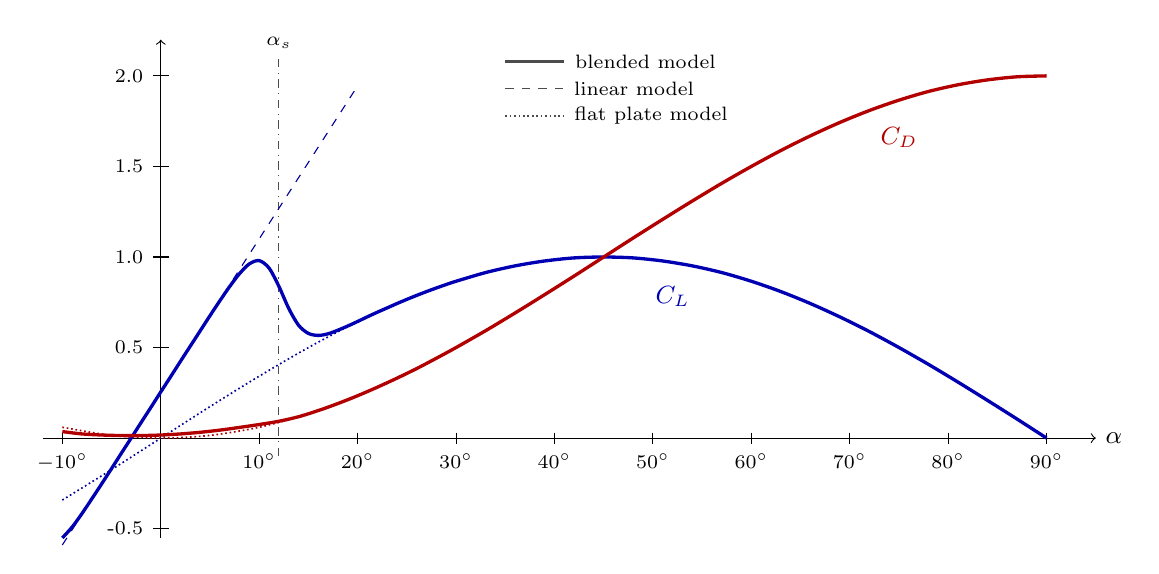
\begin{tikzpicture}[x=0.125cm, y=2.3cm, thick, every node/.style={font=\small}]
% axes
\draw[->, thin] (-12,0) -- (95,0) node[right]{$\alpha$};
\draw[->, thin] (0,-0.55) -- (0,2.2);
\foreach \a in {-10,10,20,30,40,50,60,70,80,90} {
    \draw[thin] (\a,0.03) -- (\a,-0.03) node[below, font=\scriptsize]{$\a^{\circ}$};
}
\foreach \v in {-0.5,0.5,1.0,1.5,2.0} {
    \draw[thin] (0.8,\v) -- (-0.8,\v) node[left, font=\scriptsize]{\v};
}
% stall angle
\draw[thin, dash dot, gray!60!black] (12.0,-0.1) -- (12.0,2.1) node[above, font=\scriptsize, text=black]{$\alpha_s$};
% linear and flat plate models
\draw[thin, dashed, blue!60!black] (-10,-0.590) -- (20,1.945);
\draw[semithick, densely dotted, blue!60!black] plot[smooth] coordinates {(-10,-0.342) (-5,-0.174) (0,0.000) (5,0.174) (10,0.342) (15,0.500) (20,0.643) (25,0.766) (30,0.866) (35,0.940) (40,0.985) (45,1.000)};
\draw[semithick, densely dotted, red!65!black] plot[smooth] coordinates {(-10,0.060) (-5,0.015) (0,0.000) (5,0.015) (10,0.060) (15,0.134) (20,0.234) (25,0.357) (30,0.500)};
% CL
\draw[very thick, blue!70!black] plot[smooth] coordinates {(-10,-0.551) (-9,-0.491) (-8,-0.416) (-7,-0.335) (-6,-0.252) (-5,-0.168) (-4,-0.083) (-3,0.001) (-2,0.086) (-1,0.170) (0,0.255) (1,0.339) (2,0.424) (3,0.508) (4,0.592) (5,0.676) (6,0.758) (7,0.837) (8,0.908) (9,0.962) (10,0.980) (11,0.939) (12,0.838) (13,0.716) (14,0.623) (15,0.578) (16,0.567) (17,0.576) (18,0.596) (19,0.619) (20,0.644) (21,0.670) (22,0.695) (23,0.719) (24,0.743) (25,0.766) (26,0.788) (27,0.809) (28,0.829) (29,0.848) (30,0.866) (33,0.914) (36,0.951) (39,0.978) (42,0.995) (45,1.000) (48,0.995) (51,0.978) (54,0.951) (57,0.914) (60,0.866) (63,0.809) (66,0.743) (69,0.669) (72,0.588) (75,0.500) (78,0.407) (81,0.309) (84,0.208) (87,0.105) (90,0.000)};
% CD
\draw[very thick, red!70!black] plot[smooth] coordinates {(-10,0.036) (-8,0.023) (-6,0.017) (-4,0.014) (-2,0.014) (0,0.017) (2,0.023) (4,0.032) (6,0.044) (8,0.059) (10,0.075) (12,0.093) (14,0.118) (16,0.152) (18,0.191) (20,0.234) (22,0.281) (24,0.331) (26,0.384) (28,0.441) (30,0.500) (33,0.593) (36,0.691) (39,0.792) (42,0.895) (45,1.000) (48,1.105) (51,1.208) (54,1.309) (57,1.407) (60,1.500) (63,1.588) (66,1.669) (69,1.743) (72,1.809) (75,1.866) (78,1.914) (81,1.951) (84,1.978) (87,1.995) (90,2.000)};
\node[blue!70!black, font=\small] at (52,0.78) {$C_L$};
\node[red!70!black, font=\small] at (75,1.66) {$C_D$};
% legend
\draw[very thick, black!70] (35,2.08) -- (41,2.08) node[right, font=\scriptsize, text=black]{blended model};
\draw[thin, dashed, black!70] (35,1.93) -- (41,1.93) node[right, font=\scriptsize, text=black]{linear model};
\draw[semithick, densely dotted, black!70] (35,1.78) -- (41,1.78) node[right, font=\scriptsize, text=black]{flat plate model};
\end{tikzpicture}
\caption[Lift and drag coefficients of the aerodynamic model]{Lift and drag coefficients of the aerodynamic model for the wing of the reference drone (NACA 3416 section, aspect ratio 7.5). The dashed line is the linear model \eqref{eq:aero-linear} (shown for the lift only), the dotted lines are the flat plate model \eqref{eq:aero-plate}, and the solid lines are their blend \eqref{eq:aero-blend} around the stall angle $\alpha_s = 12.0^{\circ}$ of the finite wing. The maximum lift coefficient is 0.98 and the best lift to drag ratio of the isolated wing is 18.7.}
\label{fig:aero-coefficients}
\end{figure}

The parameters of the section, $\alpha_0$, $\alpha_s^{\mathrm{2D}}$, $C_{D_0}$ and $\mathit{Re}_{\mathrm{nom}}$, are not free constants. The wing section is a four-digit NACA airfoil chosen by the genome of the body, and its parameters are read from a table that was computed in advance, for every admissible airfoil, from polars obtained with the panel code XFOIL \cite{drela1989xfoil} over a sweep of Reynolds numbers. The slope of the section is fixed at $C_{\ell_\alpha} = 0.11$ per degree, the value that thin airfoil theory predicts to within one percent. The elevator and the rudder always use the same symmetric section. The fuselage produces no lift and a constant drag coefficient of 0.35 referred to its own reference area.

\paragraph{Forces and points of application.} With the dynamic pressure $\tfrac{1}{2}\rho V^2$, the air density $\rho = 1.225$~kg/m$^3$ and the area $S$ of the element, lift and drag are
\begin{equation}
L = \tfrac{1}{2}\,\rho V^2 S\, C_L \cos^2\!\beta, \qquad D = \tfrac{1}{2}\,\rho V^2 S\, C_D \cos^2\!\beta,
\label{eq:aero-lift-drag}
\end{equation}
where the factor $\cos^2\beta$, applied to the wing and to the elevator, expresses the classical result that only the component of the flow normal to the span of a surface loads it. The two magnitudes are assembled in wind axes and rotated into the frame of the surface through the two aerodynamic angles,
\begin{equation}
\vect{F} = \mat{R}_z(\beta)\, \mat{R}_y(\alpha)\, \bigl( D,\; 0,\; L \bigr)^{\top},
\label{eq:aero-force}
\end{equation}
with $\mat{R}_y$ and $\mat{R}_z$ the elementary rotations about the $y$ and $z$ axes of the frame. The rudder is treated as a wing turned by ninety degrees: its incidence is the sideslip angle, its coefficients are evaluated at $\beta$, and its lift acts as a side force along $y$. The force is not applied at the origin of the frame but at the \emph{centre of pressure} of the surface, which for an attached flow lies at the quarter of the chord and moves towards the middle of the chord as the flow separates:
\begin{equation}
\frac{x_{\mathrm{cp}}}{\bar c} = \frac{1}{4} + \frac{1}{4}\, \frac{\lvert\alpha\rvert}{\pi/2} .
\label{eq:aero-cp}
\end{equation}
Since the rigid body solver receives a force and a point, the aerodynamic moments of the drone are never modelled as such: the pitching moment that trims the aircraft, the rolling moment of a differential twist and the yawing moment of an asymmetric sweep all arise as moments of the forces \eqref{eq:aero-force} about the centre of mass, and they change with the body because the points of application do.

\paragraph{Interaction between the elements.} Two interactions are modelled, both directed at the tail. The first is the \emph{downwash} of the wing: a wing that produces lift deflects the flow behind it downwards, and the elevator works in that deflected flow. Its angle of attack is reduced by the downwash angle that lifting-line theory predicts at the wing,
\begin{equation}
\alpha_{\mathrm{t}} = \alpha - \varepsilon, \qquad \varepsilon = k_{\varepsilon}\, \frac{C_{L,\mathrm{w}}}{\pi\, \mathit{AR}_{\mathrm{w}}},
\label{eq:aero-downwash}
\end{equation}
where $C_{L,\mathrm{w}}$ is the lift coefficient that the wing half on the same side has at that same substep, $\mathit{AR}_{\mathrm{w}}$ the aspect ratio of the wing and $k_{\varepsilon} = 1$. This couples the two surfaces the way it does on a real aircraft (an increase of wing lift reduces the effectiveness of the tail) and makes the two halves of the elevator work differently when the two halves of the wing do. For this reason the kernel evaluates the elements in a fixed order: the propeller first, then the wing and the fuselage, then the tail. The second interaction is the \emph{slipstream} of the propeller, whose induced velocity, given below, corrects the axial component of the flow seen by the elevator through a gain $k_s$.

\paragraph{Propeller.} The throttle command $u \in [0,1]$ does not set the thrust directly. It passes through a first order lag that represents the inertia of the motor and of the propeller,
\begin{equation}
\tilde u_{k+1} = \tilde u_k + \frac{\Delta t}{\Delta t + 1/(2\pi f_c)}\,\left(u_k - \tilde u_k\right),
\label{eq:prop-lag}
\end{equation}
with a cut-off frequency $f_c = 0.32$~Hz, and the filtered command sets the rotation speed $n = \tilde u\, n_{\max}$ (in revolutions per second), where $n_{\max}$ is the smaller of the no-load speed of the motor, $K_V U / 60$ for a speed constant $K_V = 2300$~rpm/V and a supply voltage $U = 7.4$~V, and of the speed at which the propeller delivers its maximum static thrust $T_{\max} = 5.2$~N. The thrust of a propeller of diameter $d$ falls as the aircraft flies faster, because the blades meet the air at a lower incidence; this is described by a thrust coefficient that decreases with the \emph{advance ratio} $J$ \cite{mccormick1995aerodynamics}:
\begin{equation}
J = \frac{V_a}{n\, d}, \qquad T = \rho\, n^2 d^4\, C_{T_0} \max\!\left(0,\; 1 - c_1 J - c_2 J^2\right),
\label{eq:prop-thrust}
\end{equation}
with $V_a$ the component of the relative wind along the axis of the propeller, $C_{T_0} = 0.093$, $c_1 = 0$ and $c_2 = 2.148$, and $T$ limited to the interval $[0, T_{\max}]$. The thrust acts along the axis, together with a reaction torque $\kappa T$ about it, $\kappa = 0.01$~m. The velocity induced in the slipstream follows from the momentum theory of the actuator disc of area $A = \pi d^2/4$:
\begin{equation}
v_{\mathrm{ind}} = \frac{1}{2}\left( -V_a + \sqrt{V_a^2 + \frac{2T}{\rho A}} \right).
\label{eq:prop-induced}
\end{equation}
The dependence of the thrust on the flight speed matters for the two objectives of this thesis. A model with a thrust proportional to the throttle would make fast flight as cheap as slow flight; with \eqref{eq:prop-thrust} the propeller loses effectiveness with speed, and the energy spent per metre depends on how well the drag of the body matches the propeller over the range of speeds at which the controller is commanded to fly.

\paragraph{Coupling and safeguards.} At each substep the forces of all elements, with their points of application, are transformed to the world frame and accumulated on the links of the rigid body as forces and moments. Three safeguards protect the explicit coupling. The speed $V$ that enters the coefficients is limited to 40~m/s, the force on each element is limited to 30~N, several times the weight of the drone, and values that are not finite are replaced by zero before they reach the rigid body solver. In a parallel simulation this last point is not cosmetic: the environments of a scene are advanced by the same kernels on shared arrays, and a single environment whose state diverges can otherwise spread its invalid values to the rest of the batch.

\paragraph{Limits of the model.} The model is a compromise between fidelity and the cost of evaluating it a hundred times per second in every environment, and its simplifications should be stated. It is quasi-steady: forces depend on the instantaneous flow only, so unsteady effects such as dynamic stall or the lag of the downwash in reaching the tail are absent. Each surface carries a single lumped force, so the distribution of the load along the span, and with it the progressive stall of a twisted or swept wing, is not resolved. The relative wind \eqref{eq:aero-angles} of every element is computed from the velocity of the centre of mass: the additional flow that a rotation of the body induces at a surface far from the centre of mass is neglected, and the rotations of the drone are damped only indirectly, through the change of incidence they produce. Interference is limited to the two effects described above. Finally, the air is at rest: there is no wind and no turbulence other than the noise described in the next subsection. None of this prevents the model from ranking bodies by the quantities that drive the search (how much wing a body has, how it is proportioned, where its surfaces sit with respect to its centre of mass, which section it uses), but the absolute values of range and energy it produces are those of the model and would need to be validated against flight data before being read as predictions.

\subsection{Simulation Noise}
\label{subsec:genesis-noise}

A deterministic simulator invites overfitting. A controller trained by reinforcement learning, and even more an evolutionary search that compares bodies by small differences in fitness, will exploit any regularity of the simulator that helps, including those that have no counterpart in reality: a lift curve known to the last digit, a centre of pressure that never wanders, a mass distribution that is exactly the nominal one. The standard countermeasure is to randomize the simulator, so that a solution can only score well if it works across a family of slightly different worlds \cite{tobin2017domain, peng2018sim}. In this thesis noise is injected at three levels of the simulation.

The first level is the aerodynamic force itself. At every physics substep, and independently for every lifting surface of every environment, the force \eqref{eq:aero-force} is perturbed in magnitude and in direction before it is applied:
\begin{equation}
\begin{gathered}
\tilde{\vect{F}} = \lVert \vect{F} \rVert \left(1 + \sigma_m\, s\, \xi\right) \frac{\hat{\vect{F}} + \sigma_d\, s\, \vect{g}_{\perp}}{\lVert \hat{\vect{F}} + \sigma_d\, s\, \vect{g}_{\perp} \rVert}, \\
s(\alpha, \beta) = 1 + 3 \left( \frac{\min\!\left(\sqrt{\alpha^2 + \beta^2},\, \pi\right)}{\pi} \right)^{\!2},
\end{gathered}
\label{eq:aero-noise}
\end{equation}
where $\hat{\vect{F}}$ is the unit vector of $\vect{F}$, $\xi$ a standard normal variable, $\vect{g}_{\perp}$ a random unit vector orthogonal to $\vect{F}$, and $\sigma_m = \sigma_d = 0.05$. The scale $s$ grows from 1 in aligned flow to 4 in fully reversed flow, so that the force is least reliable exactly where the model is: at large incidence, around and beyond stall. The centre of pressure is displaced at the same time by a random offset whose standard deviation is a fraction $\sigma_{\mathrm{cp}}\, s / 4$ of the chord, with $\sigma_{\mathrm{cp}} = 0.01$, limited to 15\% of the chord. The thrust of the propeller is not perturbed. Being drawn anew a hundred times per second, this noise acts on the drone as a broadband buffeting: its effect on the trajectory partly averages out, but it denies the controller a perfectly repeatable response to its commands.

The second level is the body. At the beginning of every flight the mass of each link is multiplied by a factor drawn from a normal distribution with mean one and standard deviation 2\%, and its centre of mass is displaced along each axis by a normal offset of standard deviation 4~mm. Both remain fixed for the duration of the flight. Genesis supports these perturbations natively: although the environments of a scene share one model, the mass and the centre of mass of every link carry an offset that is specific to the environment. For a winged drone the position of the centre of mass relative to the wing decides the stability of the aircraft, so a few millimetres are a meaningful disturbance, of the size that a real airframe shows from one assembly to the next.

The third level is the interface between the simulator and the controller: the observations are corrupted by sensor noise, the commands reach the servomotors with a random latency of up to one control step and with a small random offset, and the forest and the initial conditions are drawn at random for every flight. These belong to the definition of the task rather than to the simulator and are described with it.

The consequence is that the outcome of a flight, and therefore every quantity derived from it, is a random variable, by design and, as noted above, also because of the arithmetic of the GPU. A single flight says little about a body or about a controller. Throughout this thesis performance is an average over many flights in different forests, and the comparisons between bodies and between methods are made with that variability in view.

\section{Flight Environment}
\label{sec:flight-environment}

The task is the same in every experiment of this thesis: fly forward through a forest, as far as possible. The forest stands in a straight corridor. With $x$ the direction of flight, $y$ the lateral direction and $z$ the vertical, the corridor is $W = 100$~m wide ($\lvert y \rvert \le 50$~m), the trees occupy the stretch $0 \le x \le L$, and the drone is released 30~m before the first tree, on the axis of the corridor, 15~m above the ground and heading along $x$. A tree is a vertical cylinder of radius $r = 0.75$~m and is treated as infinitely tall, so that a forest cannot be flown over: avoiding the trees is a planar problem, and the altitude matters only to the flight itself.

As anticipated in \autoref{subsec:genesis-physics}, the trees are not objects of the physics engine. A forest is nothing more than the list of the positions of its trunks, and a batch of $F$ forests of $T$ trees each is a single tensor of $F \times T$ positions that resides on the GPU. At the beginning of every flight an environment is assigned one of the $F$ forests, and from then on the forest enters the simulation through two operations only, which are computed for all environments at once: what the drone sees, which is described with its sensors in \autoref{subsec:drone-sensors}, and whether it has hit something.

\paragraph{Collision.} Let $(x_b, y_b)$ be the position of the centre of a trunk in the horizontal frame centred on the drone and aligned with its heading, $b$ the combined span of the two wing panels (1.4~m for the reference drone, whose wing measures 1.5~m from tip to tip once the fuselage between the panels is counted) and $\phi$ its roll angle. The drone has hit the trunk when
\begin{equation}
\lvert x_b \rvert \le r + \tau \qquad \text{and} \qquad \lvert y_b \rvert \le \frac{b}{2}\cos\phi + r + \tau ,
\label{eq:forest-collision}
\end{equation}
that is, when the trunk overlaps the segment that the wing projects on the ground, which shortens as the drone banks (the rectangle is drawn in \autoref{fig:forest-sensing}). A drone can therefore pass through a gap narrower than its wingspan, but only by rolling steeply while it does so. The test is an approximation: it ignores the width of the fuselage, the length of the body and the sweep of the panels. The margin $\tau$ is 1~cm when a body is evaluated and 20~cm during the training of the controllers, which teaches them to keep some distance from the trunks.

\paragraph{End of a flight.} A flight ends when the drone hits a trunk, leaves the corridor sideways, descends to the ground, exceeds a quarter of a turn in roll, pitch or yaw (it has tumbled, or turned back), flies past the end of the forest, or reaches a time limit. The coordinate $x$ at which the flight ends is its \emph{progress}, the first of the two quantities by which bodies and controllers are judged in this thesis; the second is the energy spent per metre.

What remains to be defined is how the positions of the trunks are drawn, and the choice is less innocent than it seems, because the forest decides what the progress of a flight measures. Three generators were written in the course of this work. They share the corridor and the trees described above and differ only in the law of the positions: one was used for internal tests, one produced every result of this thesis, and one was explored and then abandoned. The three are shown below in the same corridor and with nearly the same number of trees, so that the figures can be compared directly. The lengths and densities used in the experiments are given with the method.

\subsection{Uniform Density Forests}
\label{subsec:forest-uniform}

The simplest forest places a fixed number $N$ of trees independently and uniformly in the rectangle $[0, L] \times [-W/2, W/2]$ (\autoref{fig:forest-uniform}). The density is the same everywhere, $N/(LW)$ trees per square metre, or, in the unit used throughout this section, $\lambda = N/L$ trees per metre of course.

\begin{figure}[htbp]
\centering
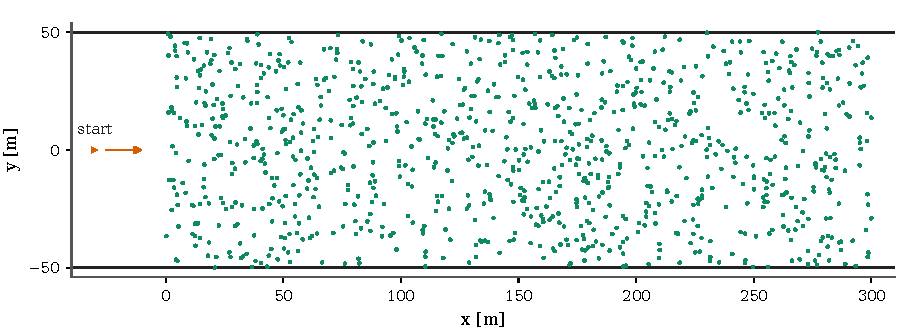
\includegraphics[width=\textwidth]{images/04_Simulation_Environment/forest_uniform.pdf}
\caption[A uniform density forest]{A uniform density forest seen from above: 975 trees placed independently and uniformly in a corridor of 300~m by 100~m. Trunks are drawn to scale. The thickets and the clearings are not designed: they are what independent positions look like.}
\label{fig:forest-uniform}
\end{figure}

A uniform forest is statistically the same at every point of the course, and this is what makes it useful for testing. It was used to verify the depth sensor and the collision test, to debug the flight of new bodies, and to observe how a controller behaves at one given density, without the confounding effect of a forest that changes as the drone advances.

The same property makes it a poor instrument for measuring. The difficulty of a uniform forest is a single number that has to be chosen in advance, and no choice suits a population of bodies of very different ability: in a sparse forest every competent body reaches the end and the progress saturates, in a dense one they all fail within a few metres. Between these extremes the measure is dominated by chance. The cleanest way to see it is to consider a drone that flies straight and blind. It touches a trunk whenever a centre falls in the strip of width $w = b + 2r$ swept by its wing, and since the positions are independent, the probability that it is still flying at $x$ is
\begin{equation}
S(x) = \exp\!\left( -\frac{w}{W} \int_0^x \lambda(\xi)\, d\xi \right),
\label{eq:forest-survival}
\end{equation}
which for a constant $\lambda$ is an exponential law: the risk of the next metre is the same whatever the distance already flown, and the distance covered has a standard deviation equal to its mean. In the forest of \autoref{fig:forest-uniform}, with $b = 1.4$~m for the reference drone, that mean is 11~m. A controller that sees the trees does much better than this, but it inherits the structure of the problem: in a stationary forest the length of a flight has a large memoryless component, and many flights are needed before two bodies can be told apart.

\subsection{Growing Density Forests}
\label{subsec:forest-growing}

In the forests used for all the results of this thesis the density grows linearly along the course, from $\lambda_0$ trees per metre at the entrance to $\lambda_1$ at the end:
\begin{equation}
\lambda(x) = \lambda_0 + (\lambda_1 - \lambda_0)\,\frac{x}{L} .
\label{eq:forest-density}
\end{equation}
The number of trees is the integral of the profile, $N = \lceil (\lambda_0 + \lambda_1) L / 2 \rceil$. The lateral coordinate of each tree is uniform across the corridor, as before, and its coordinate along the course is drawn from the density proportional to \eqref{eq:forest-density} by inverting its cumulative distribution, which for a linear profile has a closed form: if $u$ is uniform in $[0,1]$,
\begin{equation}
x = L\; \frac{\sqrt{\lambda_0^2 + u\left(\lambda_1^2 - \lambda_0^2\right)} - \lambda_0}{\lambda_1 - \lambda_0} .
\label{eq:forest-inverse-cdf}
\end{equation}
A whole batch of forests is thus generated with a handful of tensor operations. The entrance density $\lambda_0$ can also be drawn at random for each forest within a given range, an option used during training so that the controller meets dense forest at the beginning of a flight as well as at the end. Since the forests of a batch share one tensor and may have different numbers of trees, the shorter lists are padded with inactive trees parked outside the corridor, where they can be neither seen nor hit. \autoref{fig:forest-growing} shows one forest and its profile.

\begin{figure}[htbp]
\centering
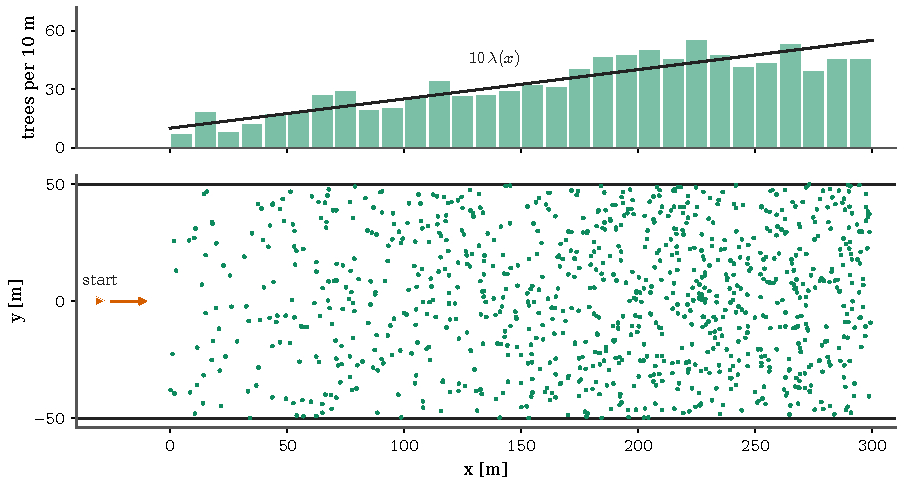
\includegraphics[width=\textwidth]{images/04_Simulation_Environment/forest_growing.pdf}
\caption[A growing density forest]{A growing density forest seen from above, with $\lambda_0 = 1$ and $\lambda_1 = 5.5$ trees per metre over 300~m, which gives the same number of trees, 975, as in \autoref{fig:forest-uniform}. The upper panel counts the trees in each 10~m of course and compares them with the profile \eqref{eq:forest-density}.}
\label{fig:forest-growing}
\end{figure}

The reason for this design is what it does to the measure. A growing forest is a course of increasing difficulty, and every flight, of whatever body, ends where the forest has become too dense for it: the progress of a flight reads directly as the density that the pair of body and controller can cope with. A single course therefore ranks the weak and the strong alike, the former in its first part and the latter in its last, and as long as the course is long enough that nobody reaches its end, the measure does not saturate. The role of chance shrinks as well. With the profile \eqref{eq:forest-density} the survival \eqref{eq:forest-survival} of the blind straight flight becomes
\begin{equation}
S(x) = \exp\!\left[ -\frac{w}{W} \left( \lambda_0\, x + \frac{\lambda_1 - \lambda_0}{2L}\, x^2 \right) \right],
\label{eq:forest-survival-growing}
\end{equation}
whose quadratic term makes long flights rapidly improbable instead of merely rare: the risk now grows with the distance, and flights end in a band rather than anywhere. In the forest of \autoref{fig:forest-growing} the blind flight covers 26~m on average and gets past 100~m less than once in a hundred attempts. Whatever a drone achieves beyond that is owed to what it sees and to how well its body lets it act on it, which is exactly what the progress is meant to measure.

The design also helps learning. A controller at the beginning of its training crashes early and therefore only ever experiences the sparse part of the forest; as it improves it reaches denser stretches, and the difficulty of its experience grows with its competence without any schedule having to be imposed. Finally, the positions remain independent, so a growing forest keeps the irregular texture of the uniform one, with its thickets and its clearings, and this turned out to matter, as the next subsection explains.

\subsection{Latin Hypercube Forests}
\label{subsec:forest-latin}

Independent positions have a cost. Nothing prevents two trunks from being drawn on top of each other, or a few of them from lining up so closely that they form a wall. The effect is not marginal. For independent positions of areal density $n$, the probability that a tree has a neighbour closer than a distance $d$ is $1 - e^{-n\pi d^2}$: at one tree every 25~m$^2$, a density that the forests of this work reach in their last part, a quarter of the trunks overlap another trunk ($d = 2r$), and almost two thirds are separated from their nearest neighbour by a gap narrower than the width $b$ of the reference drone ($d = 2r + b$). Chains of such pairs form barriers several metres wide (\autoref{fig:forest-overlaps}, left). A flight that ends against one of them says little about the body or about the controller, and this luck of the draw is one of the sources of the noise that every comparison in this thesis has to average out.

\begin{figure}[htbp]
\centering
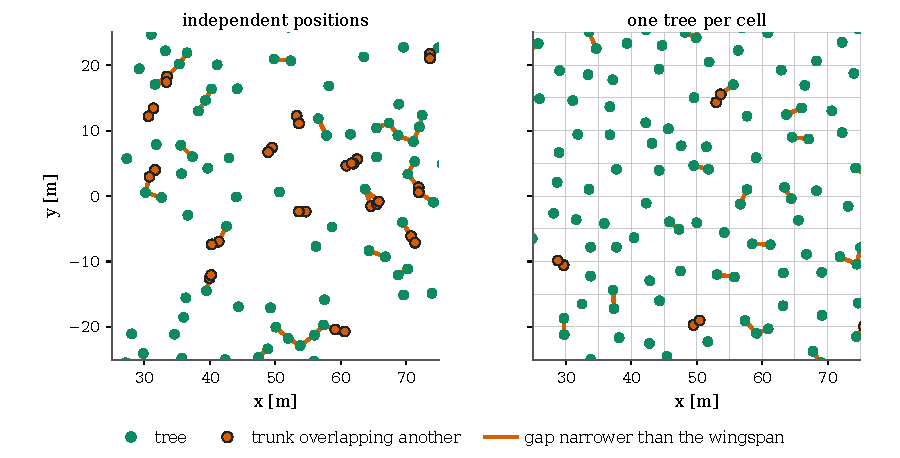
\includegraphics[width=\textwidth]{images/04_Simulation_Environment/forest_random_vs_stratified.pdf}
\caption[Independent and stratified positions at the same density]{Independent and stratified positions at the same density, one tree every 25~m$^2$, in a window of 50~m by 50~m with trunks to scale. With independent positions 25\% of the trunks overlap another and 64\% leave a gap narrower than the width $b = 1.4$~m of the reference drone; with one tree per cell the two figures fall to 6\% and 39\% (averages over 200 forests).}
\label{fig:forest-overlaps}
\end{figure}

The third generator was written to remove this effect. It borrows the idea of \emph{Latin hypercube sampling} \cite{mckay1979comparison}, the classical device for spreading random samples evenly over a domain: the domain is divided into strata and the samples are forced to occupy them evenly, while remaining random inside them. Here the corridor is tiled with rectangular cells and exactly one tree is placed in each cell, at a position uniform within it. To keep the density growing along the course, the cells shrink: the course is cut into columns whose width decreases linearly from $s_0$ at the entrance to $s_1$ at the end (the widths being rescaled so that they tile the length $L$ exactly), and each column is cut into equal rows whose height follows the same interpolation (\autoref{fig:forest-latin}). The name is used loosely. In a Latin hypercube proper each row and each column of the grid holds exactly one sample; here every cell does, which is the stronger form of stratification also known as jittered sampling.

\begin{figure}[htbp]
\centering
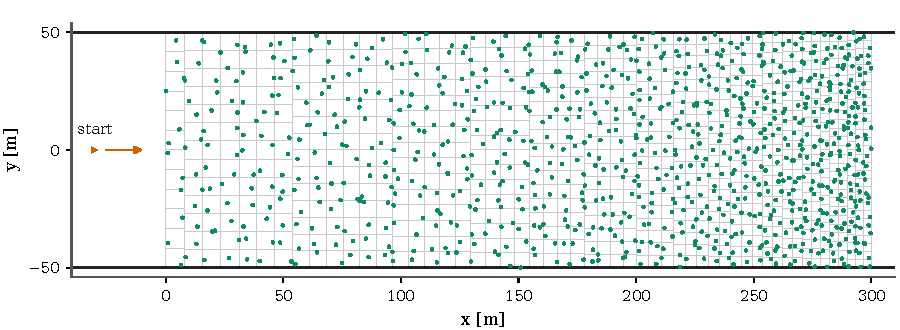
\includegraphics[width=\textwidth]{images/04_Simulation_Environment/forest_latin.pdf}
\caption[A Latin hypercube forest]{A Latin hypercube forest seen from above, with its cells. The cells shrink from 8~m to 3.4~m along the course and each holds exactly one tree, for 988 trees in total, about as many as in \autoref{fig:forest-uniform} and \autoref{fig:forest-growing}.}
\label{fig:forest-latin}
\end{figure}

The stratification does what it was meant to do. At the same density the overlapping trunks fall from 25\% to 6\% and the gaps narrower than the width $b$ from 64\% to 39\% (\autoref{fig:forest-overlaps}, right); no region can be crowded, because at most four trees can meet around the corner shared by four cells, and none can be empty, because every cell is occupied. The number of trees is also identical in all the forests of a batch, which removes the need for padding.

It was nevertheless abandoned, because what it removes is part of the task. A forest drawn in this way is tidy: the trees are almost evenly spaced, every gap is about one cell wide, and the thickets and the clearings that a real forest has, and that \autoref{fig:forest-uniform} and \autoref{fig:forest-growing} show, are gone. A body and a controller selected in such a forest are selected in the presence of a regularity that no real environment offers, and a search could come to rely on it. Deciding when to go around a thicket and when to cut through a clearing is, on the contrary, part of what flying through a forest means. The choice made in this thesis is therefore to keep the forest natural and to pay for its luck with numbers: the results are obtained in growing density forests with independent positions, and the chance of an unlucky forest is averaged out over many of them.

\section{Drone Model}
\label{sec:drone-model}

The body that flies through the forest is a small electric aircraft with a morphing wing. It is not a fixed model: every body is generated by a script that turns a genome of fifteen numbers into a URDF file, with its geometry, its masses and inertias, its joints and the reference frames of the aerodynamic solver of \autoref{subsec:genesis-aero}. What all bodies have in common is their architecture, that is, which parts they are made of, how these are actuated and what the drone can sense; what distinguishes them is the size, the proportions and the placement of those parts. This section describes the common architecture first, then the genome, and finally the particular body that is used as the reference throughout the thesis.

\subsection{Drone Shape and Actuators}
\label{subsec:drone-shape}

The drone has a conventional layout (\autoref{fig:drone-actuators}). A straight fuselage of constant cross-section, 10~cm wide, carries a propeller of 10~cm radius at its nose, a wing made of two independent rectangular panels attached to its sides, and a tail at its rear end formed by a horizontal surface, the elevator, and a vertical one, the rudder. The fuselage also houses the battery, the electronics and a small camera at the nose, which are fixed masses.

What is not conventional is the way the drone is controlled. There are no ailerons, no flaps and no hinged control surfaces of any kind: the surfaces move as a whole. Each wing panel is connected to the fuselage by two revolute joints in series that share the same point at its root, on the quarter-chord line. The first rotates the panel about the vertical axis and changes its \emph{sweep}; the second rotates it about its own spanwise axis and changes its \emph{twist}, that is, its incidence. The elevator is a single all-moving surface that pitches about a hinge at the end of the fuselage, and the rudder is an all-moving fin that turns about a vertical axis mounted on the elevator, so that it pitches with it. Together with the throttle of the propeller, this gives the seven commands that a controller issues at every control step:
\begin{equation}
\vect{a} = \left( u,\; \delta^{\mathrm{sw}}_{\mathrm{L}},\; \delta^{\mathrm{sw}}_{\mathrm{R}},\; \delta^{\mathrm{tw}}_{\mathrm{L}},\; \delta^{\mathrm{tw}}_{\mathrm{R}},\; \delta^{\mathrm{el}},\; \delta^{\mathrm{ru}} \right),
\label{eq:drone-actions}
\end{equation}
the throttle $u \in [0,1]$ and six target angles, each bounded by the mechanical range of its joint. The two panels are commanded independently, so the wing can be moved symmetrically, to trim the aircraft and to change its lift, or asymmetrically, to roll and to turn: a differential twist does the work of the ailerons of a conventional aircraft. This is the kind of morphing wing studied for winged drones by Bergonti et al. \cite{bergonti2024codesign}, here combined with a moving tail.

\begin{figure}[htbp]
\centering
\begin{subfigure}[c]{0.44\textwidth}
\centering
\begin{tikzpicture}[>={Stealth[length=2mm]}, thick, scale=0.92, transform shape, every node/.style={font=\scriptsize}]
\tikzset{
  part/.style={draw=black!65, fill=black!8, rounded corners=1.5pt},
  joint/.style={draw=orange!60!black, fill=orange!35, circle, inner sep=0pt, minimum size=5pt},
  tag/.style={draw=orange!60!black, fill=orange!14, rounded corners=1.5pt, inner sep=2.2pt, align=center},
}
% fuselage, propeller
\draw[part] (-0.22,-2.2) rectangle (0.22,2.0);
\draw[part, fill=black!55] (-0.85,2.06) rectangle (0.85,2.2);
\draw[->, orange!60!black, very thick] (0,2.3) -- (0,2.95);
\node[tag, anchor=west] at (0.3,2.72) {throttle $u$};
% wing panels
\draw[part] (-2.95,0.55) rectangle (-0.42,1.25);
\draw[part] (0.42,0.55) rectangle (2.95,1.25);
\node[joint] at (-0.32,1.07) {};
\node[joint] at (0.32,1.07) {};
\node[tag] at (-1.7,0.05) {sweep $\delta^{\mathrm{sw}}_{\mathrm{L}}$, twist $\delta^{\mathrm{tw}}_{\mathrm{L}}$};
\node[tag] at (1.7,0.05) {sweep $\delta^{\mathrm{sw}}_{\mathrm{R}}$, twist $\delta^{\mathrm{tw}}_{\mathrm{R}}$};
% tail
\draw[part] (-1.25,-2.75) rectangle (1.25,-2.33);
\draw[part, fill=black!30] (-0.06,-2.95) rectangle (0.06,-2.25);
\node[joint] at (0,-2.27) {};
\node[tag, anchor=west] at (0.45,-1.75) {elevator $\delta^{\mathrm{el}}$, rudder $\delta^{\mathrm{ru}}$};
\end{tikzpicture}
\caption{}
\label{fig:drone-actuators-scheme}
\end{subfigure}
\hfill
\begin{subfigure}[c]{0.54\textwidth}
\centering
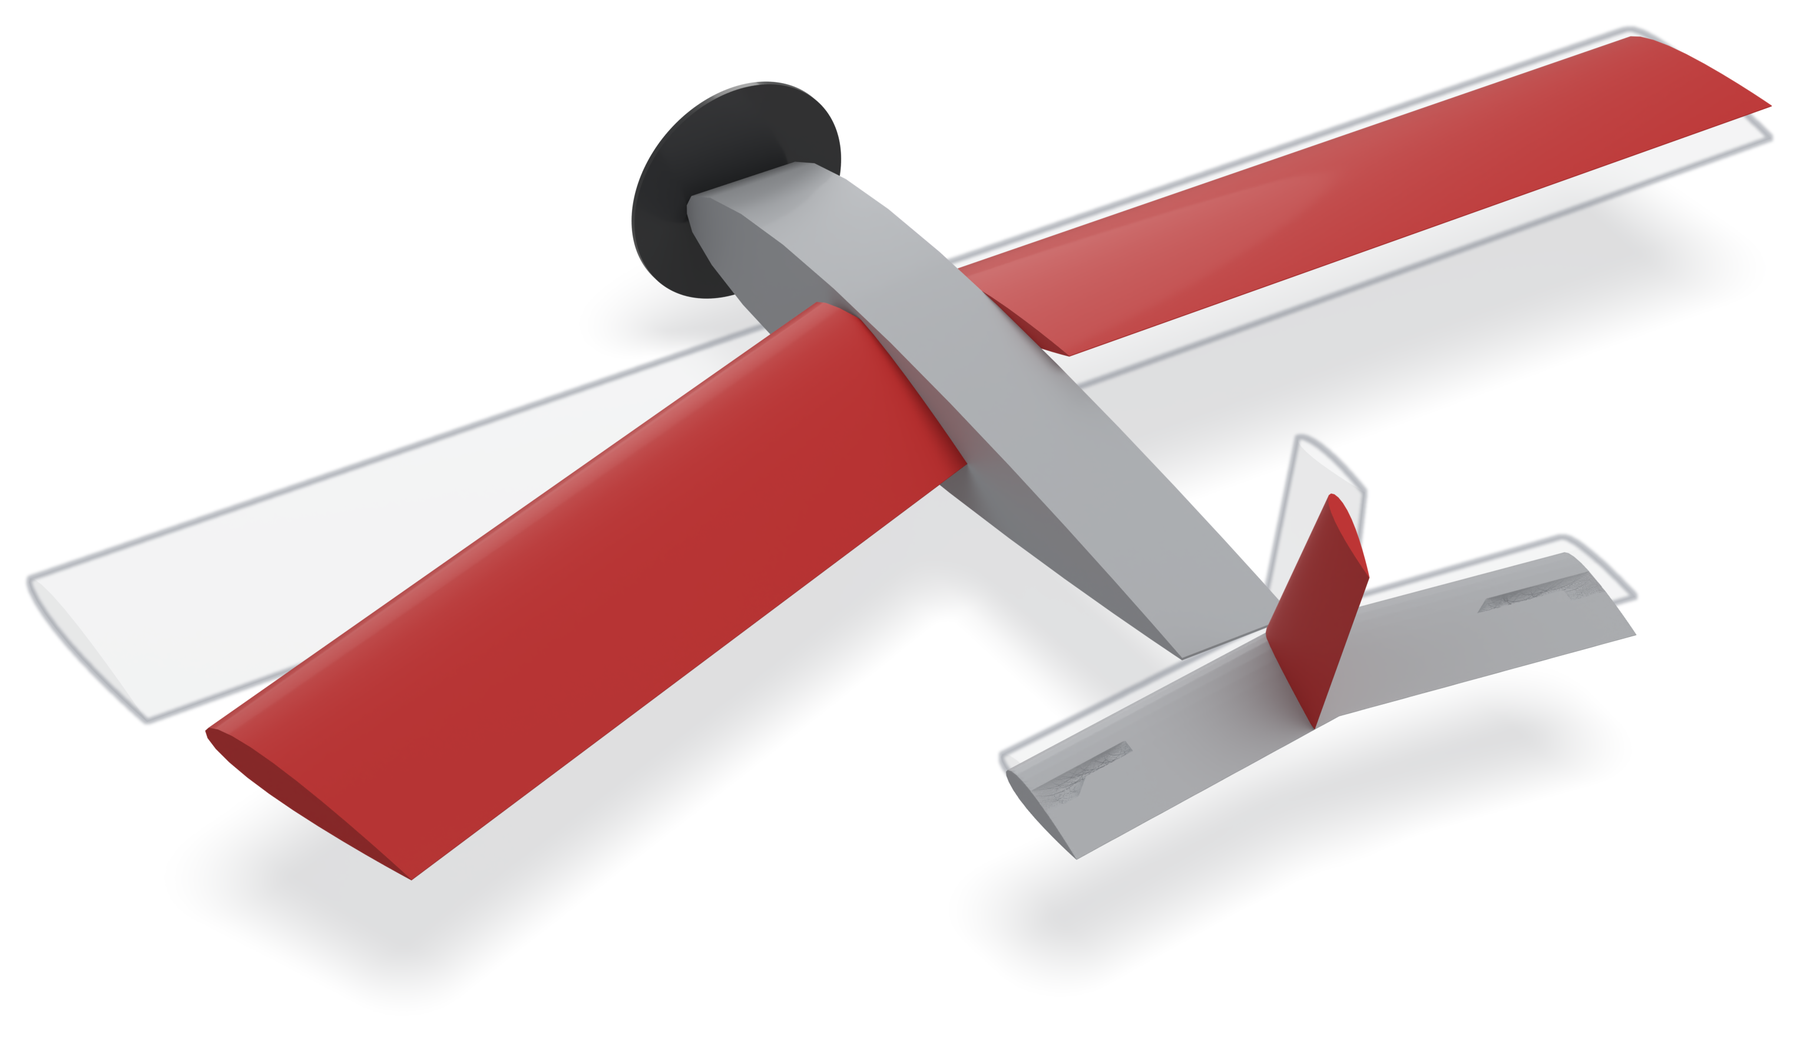
\includegraphics[width=\textwidth]{images/04_Simulation_Environment/standard_drone_actuation.png}
\caption{}
\label{fig:drone-actuators-render}
\end{subfigure}
\caption[Parts and actuators of the drone]{Parts and actuators of the drone. (a) The seven commands, on a schematic top view with the nose up: the throttle of the propeller, the sweep and the twist of each wing panel, the elevator and the rudder. (b) The reference drone with the left panel swept back to the limit of its range, the two panels twisted in opposite directions, and the elevator and the rudder deflected; the neutral position of every surface is shown in light grey.}
\label{fig:drone-actuators}
\end{figure}

\paragraph{Servomotors and gear ratios.} Every joint is driven by a servomotor, modelled as in \autoref{subsec:genesis-physics}: a position controller with a bounded torque, acting against the damping and the friction of the joint. The sweep joints use a larger servomotor than the twist and the tail joints (25~g against 10~g). Between the servomotor and a wing joint there is a reduction gear whose ratio $k$ is part of the genome, one ratio for the sweep of both panels and one for their twist. A gear trades range for strength: the panel can move within
\begin{equation}
\lvert \delta^{\mathrm{sw}} \rvert \le \frac{0.7}{k_{\mathrm{sw}}}~\text{rad}, \qquad \lvert \delta^{\mathrm{tw}} \rvert \le \frac{0.5}{k_{\mathrm{tw}}}~\text{rad},
\label{eq:drone-gear}
\end{equation}
with a torque limit of $0.75\, k_{\mathrm{sw}}$ and $0.6\, k_{\mathrm{tw}}$~N\,m respectively, while the damping and the friction felt at the joint grow with $k^2$ and with $k$. With the ratios allowed by the genome, between 1.5 and 3.5, the sweep range goes from $\pm 27^{\circ}$ to $\pm 11^{\circ}$ and the twist range from $\pm 19^{\circ}$ to $\pm 8^{\circ}$. A body can thus have a wing that moves widely but weakly, or narrowly but firmly, and which of the two is better depends on the aerodynamic loads that its panels generate, that is, on the rest of the body. The tail joints have no gear: their range is $\pm 0.25$~rad ($\pm 14^{\circ}$) and their torque limit 1~N\,m on every body. The controller never commands an angle directly: its six outputs lie in $[-1, 1]$ and are scaled by the range of the corresponding joint, so that the same output means ``full deflection'' on every body.

\paragraph{Masses.} The structure is foam. The fuselage is a shell 15~mm thick and the wing and tail surfaces are solid panels whose thickness follows their airfoil section, all with a density of 20~kg/m$^3$ (reduced by a fill factor of 0.68 for the surfaces); each part receives the mass of its volume and the inertia tensor of a box of its dimensions. To this are added the fixed masses: 200~g for the battery and the electronics, 30~g for the camera, 41.5~g for the motor and the propeller, 90~g for the six servomotors and 40~g for hinges and fittings. The fixed masses amount to about 0.40~kg and are the same for every body; the structural mass is what the genome controls. It grows quickly with the size of the wing, since the volume of a panel is proportional to the cube of its span for a given aspect ratio and section: the lightest body that the genome can express weighs 0.44~kg and the heaviest 2.5~kg, while nine bodies out of ten drawn uniformly at random weigh between 0.50 and 1.10~kg. The position of the centre of mass is controlled by a gene as well, which places the mass of the fuselage, battery included, along its length.

\paragraph{Energy.} The second quantity by which a body is judged, next to the progress of \autoref{sec:flight-environment}, is the energy it spends. The power absorbed by the propeller follows from its rotation speed $n$ and its advance ratio $J$, with the same kind of law as the thrust \eqref{eq:prop-thrust}:
\begin{equation}
P_{\mathrm{prop}} = \rho\, n^3 d^5\, C_{P_0} \max\!\left(0,\; 1 - c'_1 J - c'_2 J^2\right),
\label{eq:drone-prop-power}
\end{equation}
with $C_{P_0} = 0.044$, $c'_1 = 0$ and $c'_2 = 1.104$, which gives about 83~W at full throttle with the drone at rest. Each servomotor absorbs the mechanical power it delivers plus a resistive loss proportional to the square of its torque, and never less than zero, since a servomotor that is driven backwards by the air does not recharge the battery. Holding a panel against a steady aerodynamic load therefore costs energy even when nothing moves. No other consumption is modelled, and the losses of the motor and of its speed controller are neglected. The energy $E$ of a flight is the integral of the total power up to the end of the flight, and it is compared across bodies of different weight through the dimensionless \emph{cost of transport},
\begin{equation}
\mathit{CoT} = \frac{E}{m\, g\, \Delta x},
\label{eq:drone-cot}
\end{equation}
where $m$ is the nominal mass of the body, $g$ the acceleration of gravity and $\Delta x$ the progress of the flight: the energy spent to carry one unit of weight over one unit of distance along the corridor. Distance flown sideways or in circles adds to the energy and not to the progress, so a body that needs wide manoeuvres to get through the trees pays for them.

\subsection{Sensors}
\label{subsec:drone-sensors}

Every body carries the same sensors, and their readings are the only information about the world that a controller receives. \autoref{tab:drone-sensors} lists them. The drone knows its altitude, its attitude and its velocity, and it has a depth sensor that looks ahead. It does not know where it is along or across the corridor, it has no measure of its angular rates, of its airspeed or of the angles of its own joints, and no sensor tells it which body it is flying. The measurements are delivered at the control rate of 25~Hz and each is corrupted by Gaussian noise, as anticipated in \autoref{subsec:genesis-noise}. Besides the measurements, the controller receives two quantities that are not sensed: the seven commands it issued at the previous step, and the forward speed it is asked to keep.

\begin{table}[htbp]
\centering
\begin{tabularx}{\textwidth}{>{\raggedright\arraybackslash}X c >{\raggedright\arraybackslash}X}
\hline
Quantity & Size & Noise (standard deviation) \\
\hline
Altitude above the ground & 1 & 0.1~m \\
Attitude, as a unit quaternion & 4 & 0.01 on each component \\
Linear velocity in the world frame & 3 & 0.4~m/s along the corridor, 0.2~m/s on the other axes \\
Depth ahead, one value per sector & 20 & 1.5~m \\
\hline
Commands issued at the previous step & 7 & none \\
Commanded forward speed & 1 & none \\
\hline
\end{tabularx}
\caption[Sensors of the drone]{What the controller receives at every control step: 28 measurements, with the noise added to each, and 8 quantities that are not measured, for 36 numbers in total.}
\label{tab:drone-sensors}
\end{table}

\paragraph{Depth sensor.} The depth sensor is what lets the drone see the forest. It looks forward in the horizontal plane: a fan of $80^{\circ}$ centred on the heading is divided into 20 equal sectors, and each sector reports the distance to the surface of the nearest trunk that falls inside it, even partially, or to the lateral wall of the corridor if that is closer, up to a range of 30~m (\autoref{fig:forest-sensing}). When the drone banks, the fan narrows by the cosine of the roll angle, as the horizontal footprint of a sensor fixed to the body would. The result is a one-dimensional depth image of 20 pixels, a deliberately poor sensor: it has no vertical resolution, its range is about two seconds of flight, and a trunk hidden behind another is invisible until the first has been passed. The sensor is one of the custom Taichi kernels mentioned in \autoref{subsec:genesis-proscons}: one GPU thread for each pair of environment and sector, with an inner loop over the trees of that environment.

\begin{figure}[htbp]
\centering
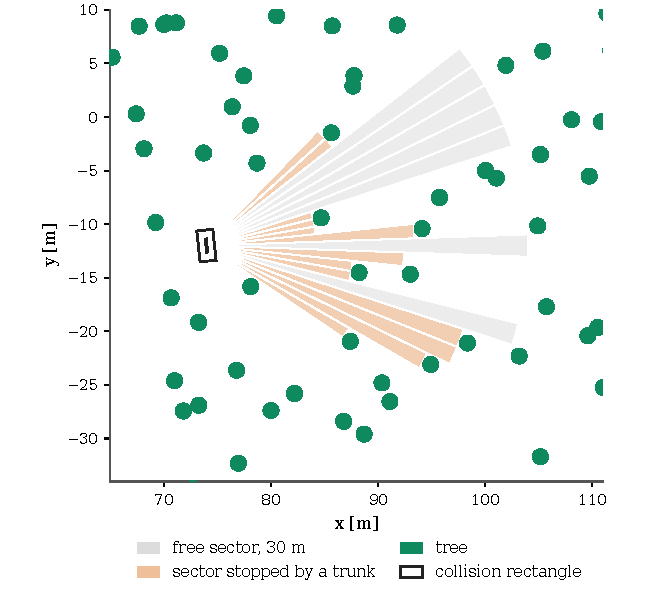
\includegraphics[width=0.74\textwidth]{images/04_Simulation_Environment/forest_sensing.pdf}
\caption[Depth sectors and collision rectangle]{What the forest is to the drone, seen from above. The depth sensor divides a fan of $80^{\circ}$ ahead of the drone into 20 sectors and reports for each the distance to the nearest trunk, up to 30~m. The collision test of \autoref{sec:flight-environment} asks whether the centre of a trunk lies inside the rectangle drawn around the wing (trunks and wingspan are to scale).}
\label{fig:forest-sensing}
\end{figure}

\subsection{Drone Genome}
\label{subsec:drone-genome}

A body is a point in a space of fifteen parameters, its \emph{genome} (\autoref{tab:drone-genome}). Each gene is stored as a number in $[0,1]$, the form in which the evolutionary algorithms handle it, and is mapped linearly onto the physical range of its parameter when the body is built. Twelve genes are continuous. The remaining three select the wing section among the four-digit NACA airfoils and are discrete: the unit interval is divided into as many equal bins as there are admissible values, and the gene takes the value of the bin it falls in.

\begin{table}[htbp]
\centering
\begin{tabularx}{\textwidth}{r >{\raggedright\arraybackslash}X c c}
\hline
 & Gene & Range & Reference drone \\
\hline
1 & Span of one wing panel & 0.4 to 0.9~m & 0.7~m \\
2 & Aspect ratio of one wing panel (span over chord) & 1.5 to 5 & 3.5 \\
3 & Length of the fuselage & 0.4 to 0.9~m & 0.73~m \\
4 & Position of the mass of the fuselage, as a fraction of its length from the nose & 0.30 to 0.60 & 0.38 \\
5 & Position of the wing root, as a fraction of the fuselage length from the nose & 0.30 to 0.60 & 0.38 \\
6 & Span of the elevator & 0.2 to 0.6~m & 0.5~m \\
7 & Aspect ratio of the elevator & 1.5 to 4 & 4 \\
8 & Span of the rudder & 0.1 to 0.4~m & 0.2~m \\
9 & Aspect ratio of the rudder & 1.5 to 4 & 2 \\
10 & Dihedral angle of the wing panels & $-4^{\circ}$ to $4^{\circ}$ & $0^{\circ}$ \\
11 & Gear ratio of the sweep joints & 1.5 to 3.5 & 2 \\
12 & Gear ratio of the twist joints & 1.5 to 3.5 & 2.5 \\
13 & Airfoil: maximum camber (first NACA digit) & 0 to 4 & 3 \\
14 & Airfoil: position of the maximum camber (second digit) & 2 to 5 & 4 \\
15 & Airfoil: thickness (last two digits) & 10 to 20 & 16 \\
\hline
\end{tabularx}
\caption[Genome of the drone]{The genome of the drone: fifteen genes, their physical ranges, and the values of the reference drone of \autoref{subsec:drone-standard}. The last three genes are discrete.}
\label{tab:drone-genome}
\end{table}

The first two genes define the wing. Its panels are rectangular, and the genes give the span $b_p$ of one panel and its aspect ratio, from which the chord is $\bar c = b_p / \mathit{AR}_p$. The wing as a whole is what these numbers imply once the two panels are mounted on the sides of a fuselage of width $w_f = 0.1$~m: a span of $2 b_p + w_f$ from tip to tip, between 0.9 and 1.9~m, and an aspect ratio of $(2 b_p + w_f)/\bar c$, which is the one that enters the aerodynamic model (\autoref{subsec:genesis-aero}) and which for the reference drone is 7.5. The same construction holds for the elevator, whose gene is its total span, while the rudder is a single panel. Genes 3 to 5 lay the aircraft out along its axis: the length of the fuselage sets the lever arm of the tail, which sits at its end, and the positions of the wing and of the mass of the fuselage along it decide, together, how far the centre of mass lies from the point where the lift of the wing acts. This distance governs the longitudinal stability of an aircraft, and a small change of either gene can turn a docile body into one that is hard or impossible to control. The dihedral gene tilts the two panels upwards or downwards at their root, and the two gear ratios set the authority of the morphing wing, as described above.

The airfoil genes act in two ways. The thickness of the section is the thickness of the panel, and therefore changes its mass and its inertia. And the section as a whole selects a row in the table of airfoil parameters of \autoref{subsec:genesis-aero}, from which the aerodynamic solver reads the zero-lift angle, the stall angle, the parasitic drag and the nominal Reynolds number of the wing. The tail surfaces are not part of the genome in this respect: they always use the same symmetric section, 16\% thick.

No constraint is imposed on the genome beyond its ranges. The generator does not check that a body is well proportioned, that its wing and its tail do not interfere, or that it is stable: any point of the unit hypercube becomes a body, and whether that body can fly is left for the flights to decide. The ranges were chosen so that a large part of the space is flyable, but nothing prevents the search from visiting the rest.

\subsection{The Standard Drone}
\label{subsec:drone-standard}

One body is singled out as the reference of the whole thesis (\autoref{fig:drone-standard}): it is the body against which the evolved ones are compared, and the point from which the quantities of this chapter were illustrated. Its genome is the last column of \autoref{tab:drone-genome}. Its wing measures 1.5~m from tip to tip with a chord of 0.2~m and a NACA 3416 section, its fuselage is 0.73~m long for an overall length of 0.89~m, and it weighs 0.605~kg.

\begin{figure}[htbp]
\centering
\begin{subfigure}[c]{0.52\textwidth}
\centering
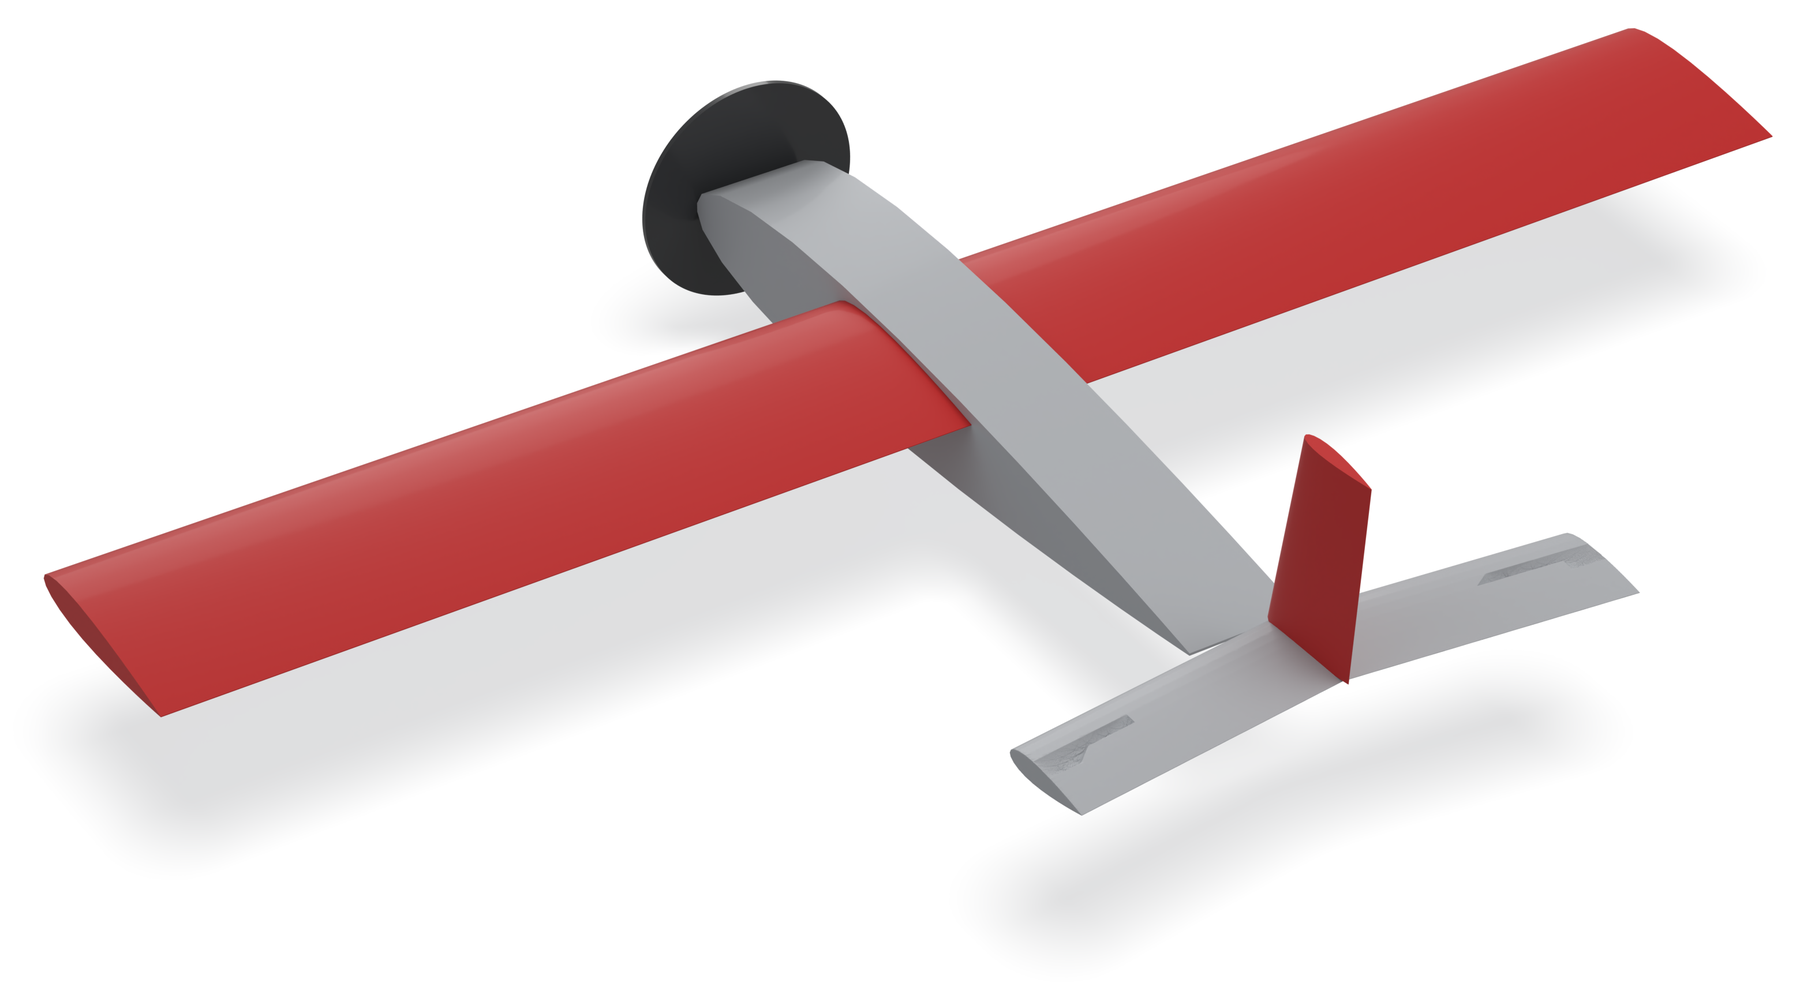
\includegraphics[width=\textwidth]{images/04_Simulation_Environment/standard_drone_neutral_3quarter.png}
\caption{}
\end{subfigure}
\hfill
\begin{subfigure}[c]{0.44\textwidth}
\centering
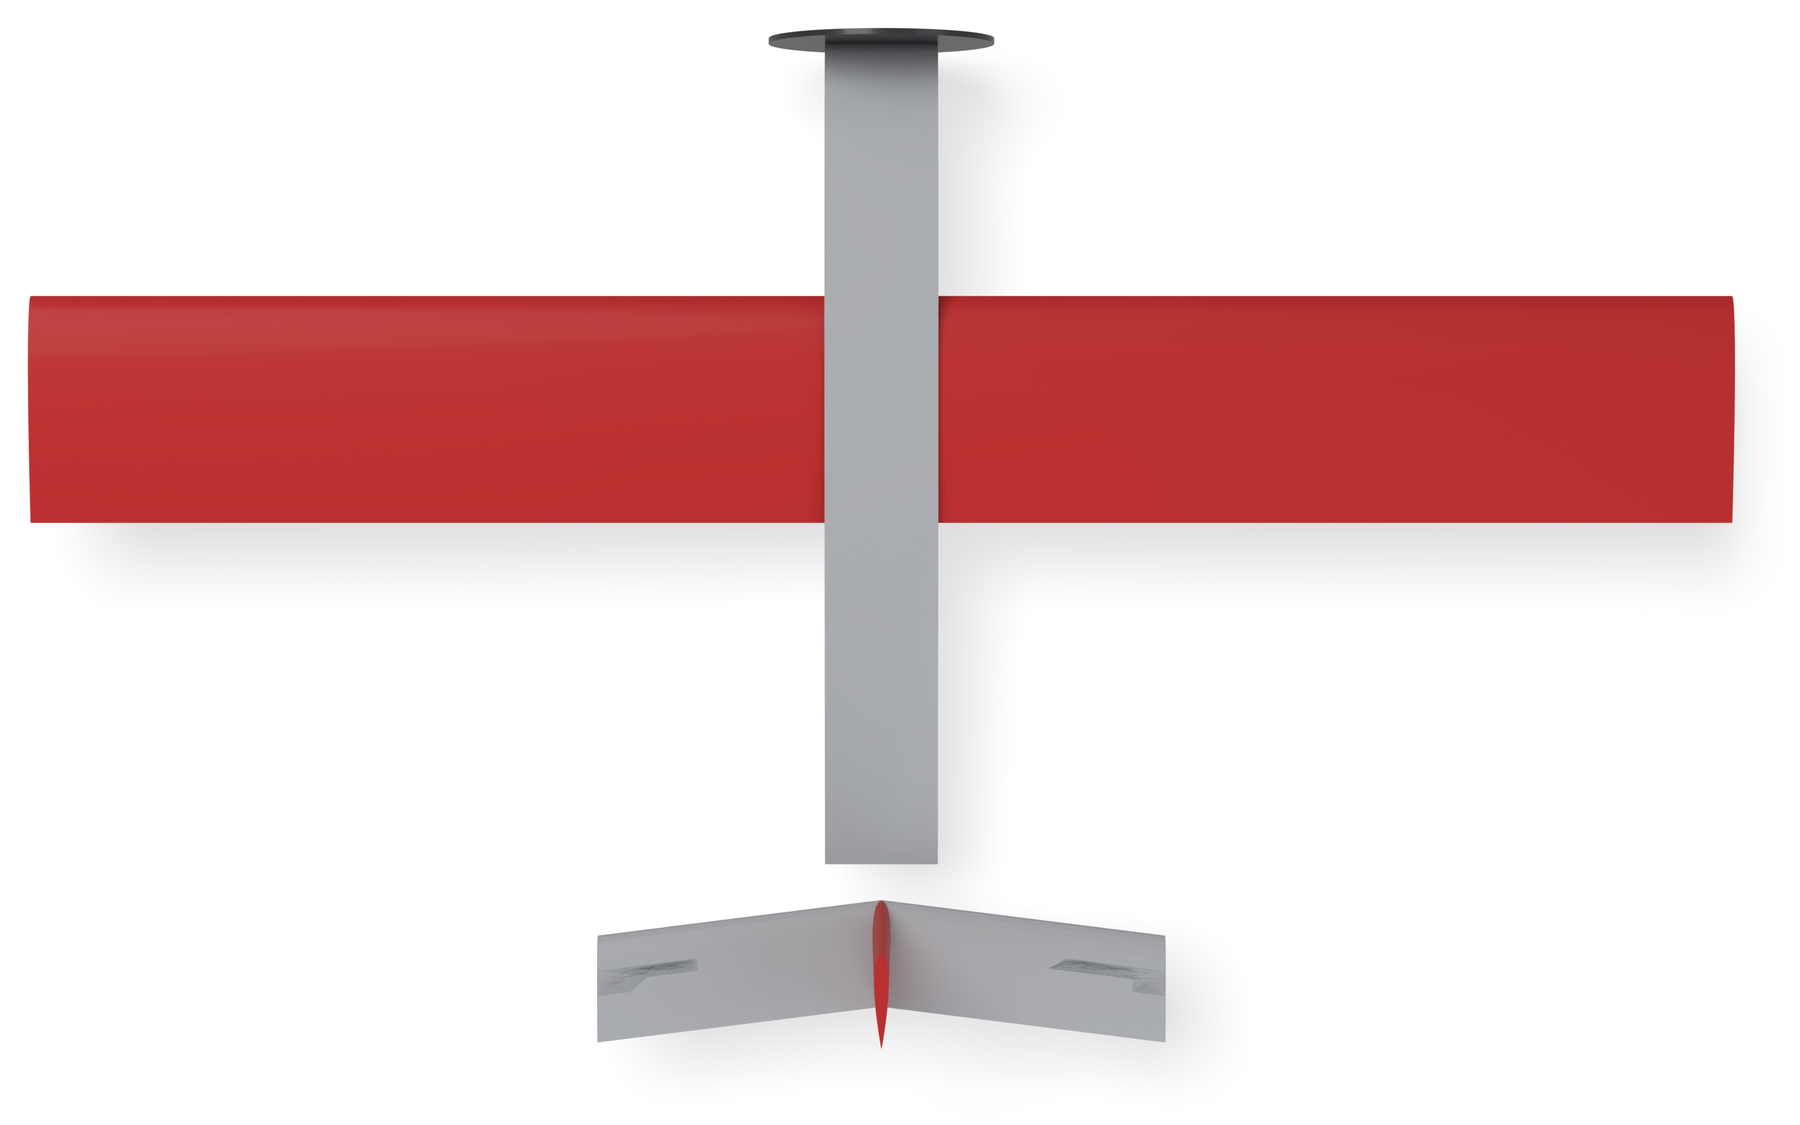
\includegraphics[width=\textwidth]{images/04_Simulation_Environment/standard_drone_neutral_top.png}
\caption{}
\end{subfigure}
\caption[The standard drone]{The standard drone with all joints in their neutral position: (a) three-quarter view, (b) top view with the nose up. The wing panels and the rudder are drawn in red, the fuselage and the elevator in grey, the disc of the propeller in black.}
\label{fig:drone-standard}
\end{figure}

These numbers are not arbitrary. The dimensions of the standard drone and the section of its wing are those of the H-King Bixler~3 \cite{hobbyking2026bixler3}, a commercial foam glider with a wingspan of 1.55~m and a length of 0.95~m that is widely used as a research platform, and that Bergonti et al. \cite{bergonti2024codesign} also adopt as the baseline of their co-design study. For this reason the figures of this thesis label the standard drone with the name of that aircraft. The correspondence, however, stops at the geometry. The Bixler~3 is flown with ailerons, an elevator and a rudder hinged on fixed surfaces, and is pushed by a propeller mounted behind its wing; the standard drone has none of those control surfaces, steers by sweeping and twisting its wing panels and by moving its tail surfaces as a whole, and is pulled by a propeller at its nose. It is also lighter, since the commercial aircraft weighs 0.89~kg ready to fly. The two aircraft share a shape, not a set of actuators, and their flight dynamics are therefore not directly comparable: the standard drone should be read as a body of familiar proportions inside the design space of \autoref{tab:drone-genome}, not as a model of the commercial aircraft.
